\documentclass[tikz,border=5pt]{standalone}
\usepackage{pgfplots}
\pgfplotsset{compat=1.18}

\definecolor{corba}{HTML}{365FB3}
\definecolor{punt}{HTML}{B91C1C}
\definecolor{guia}{HTML}{6B7280}

\begin{document}
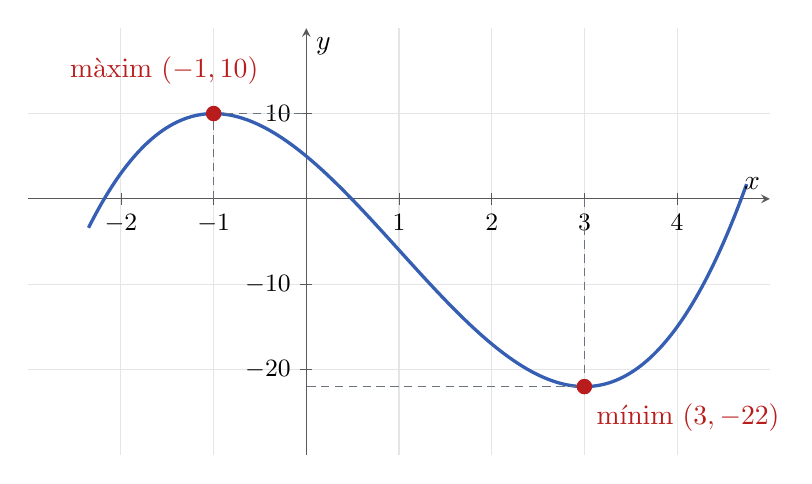
\begin{tikzpicture}
  \begin{axis}[
    width=11cm,
    height=7cm,
    axis lines=middle,
    xmin=-3,
    xmax=5,
    ymin=-30,
    ymax=20,
    xlabel={$x$},
    ylabel={$y$},
    xtick={-2,-1,0,1,2,3,4},
    ytick={-20,-10,10},
    grid=major,
    grid style={black!10},
    axis line style={black!65},
    tick style={black!65},
    tick label style={font=\small},
    clip=false,
  ]
    \addplot[corba, very thick, domain=-2.35:4.75, samples=220]
      {x^3-3*x^2-9*x+5};

    \draw[guia, densely dashed]
      (axis cs:-1,0) -- (axis cs:-1,10) -- (axis cs:0,10);
    \draw[guia, densely dashed]
      (axis cs:3,0) -- (axis cs:3,-22) -- (axis cs:0,-22);

    \addplot[only marks, mark=*, mark size=2.6pt, punt]
      coordinates {(-1,10) (3,-22)};

    \node[anchor=west, text=punt, inner sep=1.5pt]
      at (axis cs:-2.6,15) {màxim $(-1,10)$};
    \node[anchor=north west, text=punt, inner sep=1.5pt]
      at (axis cs:3.08,-23.5) {mínim $(3,-22)$};
  \end{axis}
\end{tikzpicture}
\end{document}
